\subsection{Polarisation}
Die Winkel mit den zugehörigen Intensitäten sind in Tabelle VERWEIS aufgetragen. Mit Hilfe der Funktion \textit{curve\_fit} von Python und einem First Guess von
\begin{align*}
	I_\text{guess} = \SI{100}{\micro\ampere}\sin^2(\varphi + 0.4)
\end{align*}
wird die Funktion
\begin{align*}
	I_\text{fit} = a\sin^2\left(b\varphi + c\right)
\end{align*}
an die Messwerte gefittet. Dabei ergeben sich die Parameter
\begin{align}
	a &= \SI{94+-1e-6}{\micro\ampere}
 \\
	b &= \SI{1.013+-0.006}{}
 \\
	c &= \SI{0.44+-0.02}{}
 \ .
\end{align}
Die Messwerte, der First Guess und die gefittete Funktion sind in Abbildung \ref{fig:fitPol} zu sehen.
\begin{figure}[h!]
	\centering
	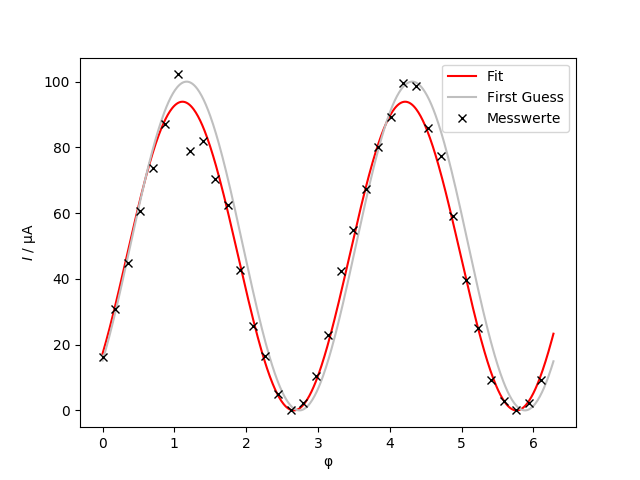
\includegraphics[width=.6\textwidth]{Fit_Polarisation.png}
	\caption{Fit zur Bestimmung der Polarisationsrichtung}
	\label{fig:fitPol}
\end{figure}
Der Laser war demnach in \SI{0.3\pi}{}
- bzw. $1.3$ - Richtung polarisiert.